\begin{frame}{Vergleich aller Modelle: Red20-Vorauswahl}
\tiny
\begin{tabular}{l r r r r l}
\toprule
Modell & GT-Faces & Treffer & Recall & ms/Bild & Rolle nach Vorauswahl \\
\midrule
FCOS R50 ep1 & 3.443 & 1.884 & 0,547 & 36,2 & Recall \\
FRCNN R50 ep1 & 3.443 & 1.714 & 0,498 & 51,4 & RCNN \\
YOLOv8m ep1 & 3.443 & 1.399 & 0,406 & 43,7 & Pipeline \\
RetinaNet ep1 & 3.443 & 1.125 & 0,327 & 35,0 & verworfen \\
\bottomrule
\end{tabular}
\end{frame}

\begin{frame}{Finaler Vergleich nach Red6/10-Training}
\tiny
\begin{tabular}{l r r r r l}
\toprule
Modell & GT-Faces & Treffer & Recall & ms/Bild & Interpretation \\
\midrule
FCOS R50 ep10 & 5.015 & 3.375 & 0,673 & 34,9 & Recall \\
YOLOv8m ep10 & 5.015 & 2.283 & 0,455 & 14,6 & Pipeline \\
FRCNN R50 ep10 & 5.015 & 3.025 & 0,603 & 49,2 & Two-Stage \\
\bottomrule
\end{tabular}

\end{frame}


\begin{frame}{Loss-Entwicklung}
\centering
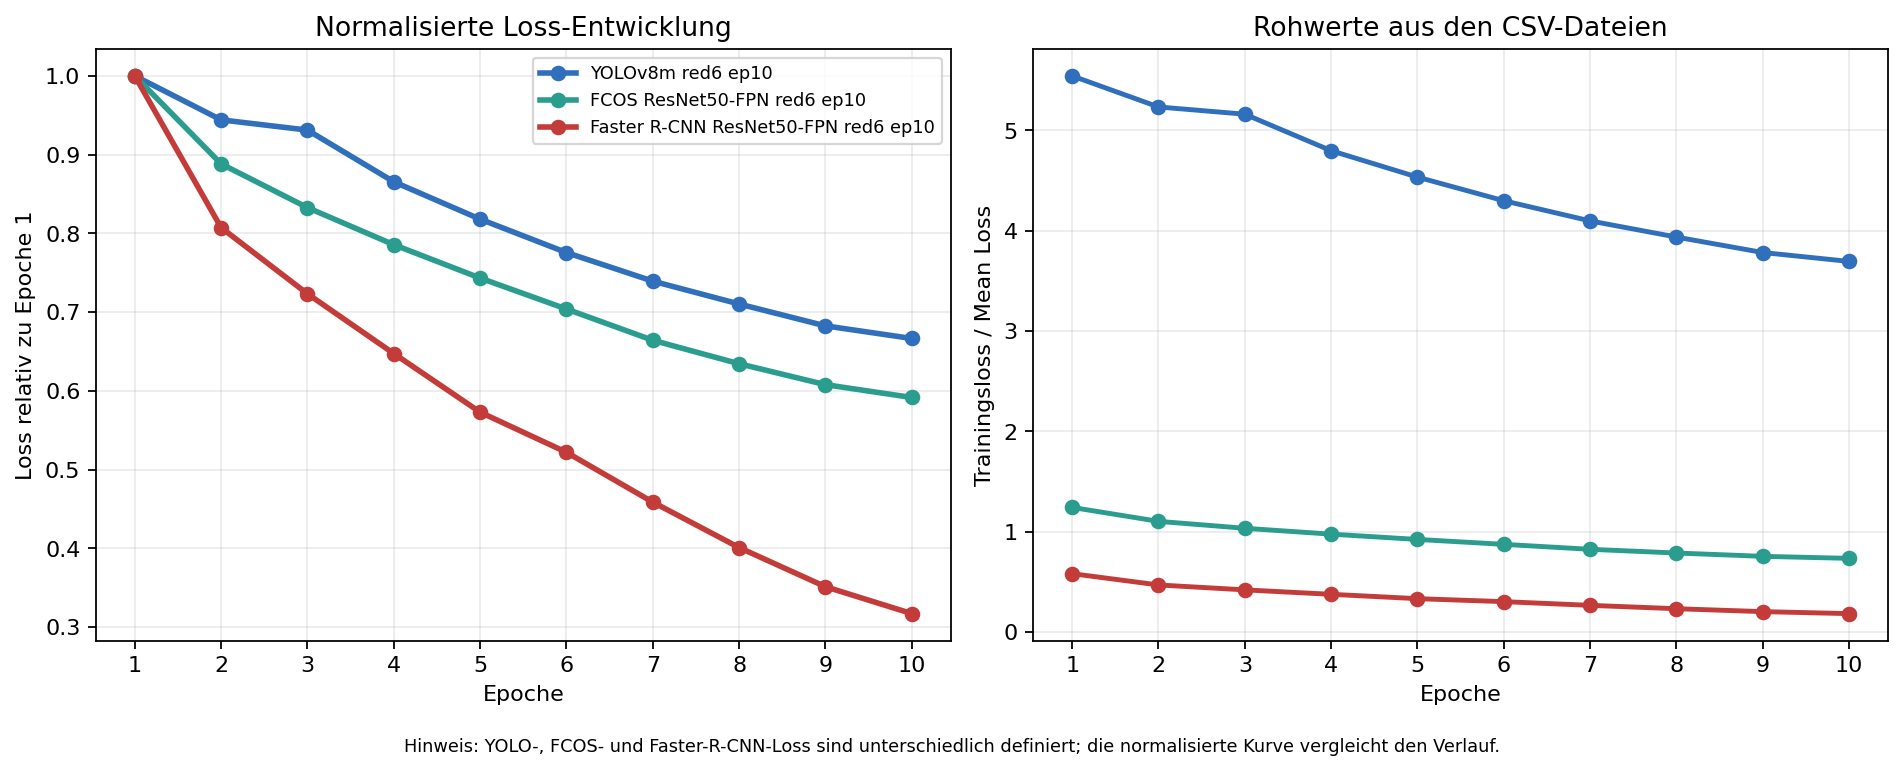
\includegraphics[width=0.96\textwidth,height=0.66\textheight,keepaspectratio]{imglib/face_model_lab/final_20260629_loss_development.png}

\vspace{0.2em}
{\tiny Roh-Loss ist je Modell anders skaliert; normalisierte Kurven zeigen den Trend.}
\end{frame}


\begin{frame}{Validierungsdurchlauf}

\small
\begin{tabular}{l r r}
\toprule
Einstellung & Red20 & Red6/10 \\
\midrule
Validierungsbilder & 300 & 500 \\
GT-Faces & 3.443 & 5.015 \\
IoU-Schwelle & 0,4 & 0,4 \\
Confidence & 0,25 & 0,25 \\
\bottomrule
\end{tabular}

\end{frame}

